\documentclass[14pt]{article}
\usepackage{tikz}

\begin{document}
  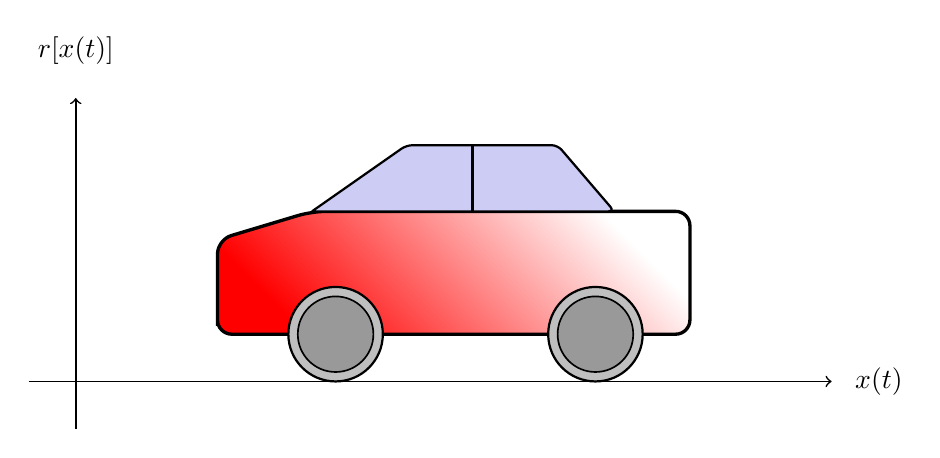
\begin{tikzpicture}[scale=1.2]
    \shade[top color=red, bottom color=white, shading angle={135}]
        [draw=black,fill=red!20,rounded corners=1.2ex,very thick] (1.5,.5) -- ++(0,1) -- ++(1,0.3) --  ++(3,0) -- ++(1,0) -- ++(0,-1.3) -- (1.5,.5) -- cycle;
    \draw[very thick, rounded corners=0.5ex,fill=black!20!blue!20!white,thick]  (2.5,1.8) -- ++(1,0.7) -- ++(1.6,0) -- ++(0.6,-0.7) -- (2.5,1.8);
    \draw[thick]  (4.2,1.8) -- (4.2,2.5);
    \draw[draw=black,fill=gray!50,thick] (2.75,.5) circle (.5);
    \draw[draw=black,fill=gray!50,thick] (5.5,.5) circle (.5);
    \draw[draw=black,fill=gray!80,semithick] (2.75,.5) circle (.4);
    \draw[draw=black,fill=gray!80,semithick] (5.5,.5) circle (.4);

    \draw[->,semithick] (0,-.5) -- (0,3);
    \draw (0,3.5) node {$r[x(t)]$};
    \draw[->,semithick] (-.5,0) -- (8,0);
    \draw (8.5,0) node {$x(t)$};
\end{tikzpicture}
\end{document}